\documentclass[10pt]{beamer}
\mode<presentation>
% \mode<handout>
{
  %\usetheme{CambridgeUS}
  \setbeamercovered{transparent}

  \definecolor{rugcolor}{rgb}{0.611, 0.188, 0.133}
  \definecolor{f1}{rgb}{1.0,1.0,1.0}
  \definecolor{f2}{rgb}{0.8, 0.0, 0.0039}
  \definecolor{b}{rgb}{0.0, 0.0, 0.0}



  \beamertemplatenavigationsymbolsempty
  \setbeamercolor{item}{fg=rugcolor!60!black}
  \setbeamercolor{structure}{fg=black}
  \setbeamercolor{title}{black}
  \setbeamercolor{item}{black}
  \setbeamercolor{frametitle}{black}



%HEADER WITH HIGHLIGHTED SECTION NAMES (optional)
  \useheadtemplate{%
    \vbox{%
        %\vskip1.2pt
        %\pgfuseimage{logo}
    %\vskip1.2pt
    \tinycolouredline{f1}{\color{white}{\bf
\insertsectionnavigationhorizontal{\paperwidth}{}{\hskip0pt plus1filll
% \pgfuseimage{logo}
}}}
\hskip0pt plus1filll
\tinycolouredline{f2}{\color{white}{\bf
\insertsubsectionnavigationhorizontal{\paperwidth}{}{\hskip0pt plus1filll
% \pgfuseimage{logo}
}}}
\flushright
\vskip1.0pt
 \pgfuseimage{logo}
}
}

% %FOOTER WITH AUTHOR NAME(S), PAPER TITLE (ABBREVIATED IF SPECIFIED BY \title),
% % AND PAGE COUNTER (optional)
%   \usefoottemplate{%
%     \vbox{%
%     \tinycolouredline{rugcolor}%
%         {\color{white}{{\insertshortauthor}\hfill%
%            \insertshorttitle\hfill%
%            \textsc{\insertframenumber/\inserttotalframenumber}
%           }}
%         }
% 
%       }
}

\pgfdeclareimage[height=0.5cm]{logo}{logo2.jpg}

\usepackage[english]{babel}
% or whatever

\usepackage[latin1]{inputenc}
% or whatever

%\usepackage{times}
%\usepackage[T1]{fontenc}
% Or whatever. Note that the encoding and the font should match. If T1
% does not look nice, try deleting the line with the fontenc.


\title[Machine Learning] % (optional, use only with long paper titles)
{
Structured Prediction\\ for Named Entity Recognition}

% \subtitle
% {Week 1} % (optional)

\author % (optional, use only with lots of authors)
{Joachim Daiber \& Carmen Klaussner}
% - Use the \inst{?} command only if the authors have different
%   affiliation.

 \institute[University of Groningen] % (optional, but mostly needed)
 {
  Information Science\\
  University of Groningen
  }
% - Use the \inst command only if there are several affiliations.
% - Keep it simple, no one is interested in your street address.

\date[Short Occasion] % (optional)
{October 24th, 2012}

%\subject{Talks}
% This is only inserted into the PDF information catalog. Can be left
% out. 



\begin{document}

\begin{frame}
  \titlepage
\end{frame}

%%%%%%%%%%%%%%%%%%%%%%%%%%%%%%%%%%%%%%%%%%%%%%%%%%%%%%


%\section{}
%\begin{frame}
%\frametitle{Motivation}
%
%% Named Entity a lot of practical uses/applications
%
%\end{frame}



%%%%%%%%%%%%%%%%%%%%%%%%%%%%%%%%%%%%%%%%%%%%%%%%%%%%




%\begin{frame}
%  \frametitle{Outline}
%  \tableofcontents
%  % You might wish to add the option [pausesections]
%\end{frame}




%%%%%%%%%%%%%%%%%%%%%%%%%%%%%%%%%%%%%%%%%%%%%%%%%

\section{Introduction}


% subsection test (end)
\begin{frame}
\frametitle{Named Entity Recognition (NER)}

\begin{figure}[htbp]
        \centering
                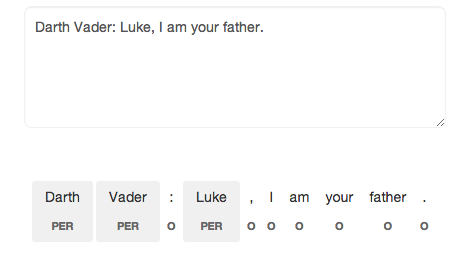
\includegraphics[scale=0.5]{figures/bsp1.png}
        \label{fig:figures_bsp1}
\end{figure}



\end{frame}


%%%%%%%%%%%%%%%%%%%%%%%%%%%%%%%%%%%%%%%%%%%%%%%%%%%%%


%\section{}
\begin{frame}
\frametitle{Entity Classes in NER}

\begin{itemize}
 \item Enamex types
\begin{itemize}
 \item Person Names: \texttt{John Bateman}
 \item Organisations: \texttt{Lavazza}
 \item Locations: \texttt{France, Bristol}
\end{itemize}

 \item Miscellaneous (CoNLL)
 \begin{itemize}
  \item  proper names outside the classic \emph{enamex}
  \item the type \emph{product}
 \end{itemize}

 \item timex (Date \& Time Expressions)
 
\item numex Monetary Values \& Percent
\end{itemize}        

$\Rightarrow$ only specific entities; \emph{in June}/ \emph{the prof} (undefined year/person) % deictic reference to sth. in previous text 
 \end{frame}

%%%%%%%%%%%%%%%%%%%%%%%%%%%%%%%%%%%%%%%%%%%%%%%%%%%%%%%%

\section{Labeled data}
\begin{frame}
\frametitle{Labeled data}


\begin{itemize}
        \item organized challenges
        \begin{itemize}
         \item CoNLL 2002/2003 
         \item Languages: English, German, Spanish \& Dutch
         \item news data 
        \end{itemize}
    \item labels: ORG / LOC/  PER/ MISC 
\end{itemize}
\end{frame}

 
%%%%%%%%%%%%%%%%%%%%%%%%%%%%%%%%%%%%%%%%%%%%%%%%%%%%%%%%


%\section{}
\begin{frame}
\frametitle{Approaches to NER}

\begin{enumerate}
 \item linguistic grammar-based techniques
 \item statistical models
\end{enumerate}

1. hand-crafted rules may obtain a high precision, but at cost of low recall
and extensive work by computational linguists\\

2. Statistical NER systems require large amount of manually annotated training data

$\Rightarrow$ supervised methods most prominent


\end{frame}


%%%%%%%%%%%%%%%%%%%%%%%%%%%%%%%%%%%%%%%%%%%%%%%%%%%%%%%%%                                        
%\section{}
\begin{frame}
\frametitle{Issues for NER}


\begin{itemize}
 \item Ambiguity


\begin{itemize}
 \item \textbf{Polysemy:} \texttt{Location} vs. \texttt{Person} \\
 
 \emph{Paris (France) - Paris (Hilton)}\\
 
 \item \textbf{Metonymy:}  (part-whole):
 
 ``\textbf{Paris} has decided to introduce an increase in tax...'' \\
 
 $\Rightarrow$ (the \textbf{government} not the \textbf{city})  
\end{itemize}

 \item mainly domain-specific systems - not readily portable to different domain/genre % drop in performance for every system (some 20% to 40% of precision and recall).
 
\end{itemize}

\end{frame}

%%%%%%%%%%%%%%%%%%%%%%%%%%%%%%%%%%%%%%%%%%%%%%%%%%%%%%%%%                

\begin{frame}[t]
\frametitle{Structured Prediction}

general framework for prediction $\mathbf{x} \rightarrow \mathbf{y}$ where $\mathbf{y}$ is structured (tree, sequence, etc.)


\begin{columns}[t]
	
	\begin{column}{.3\textwidth}

	\begin{figure}[t]
		\centering
			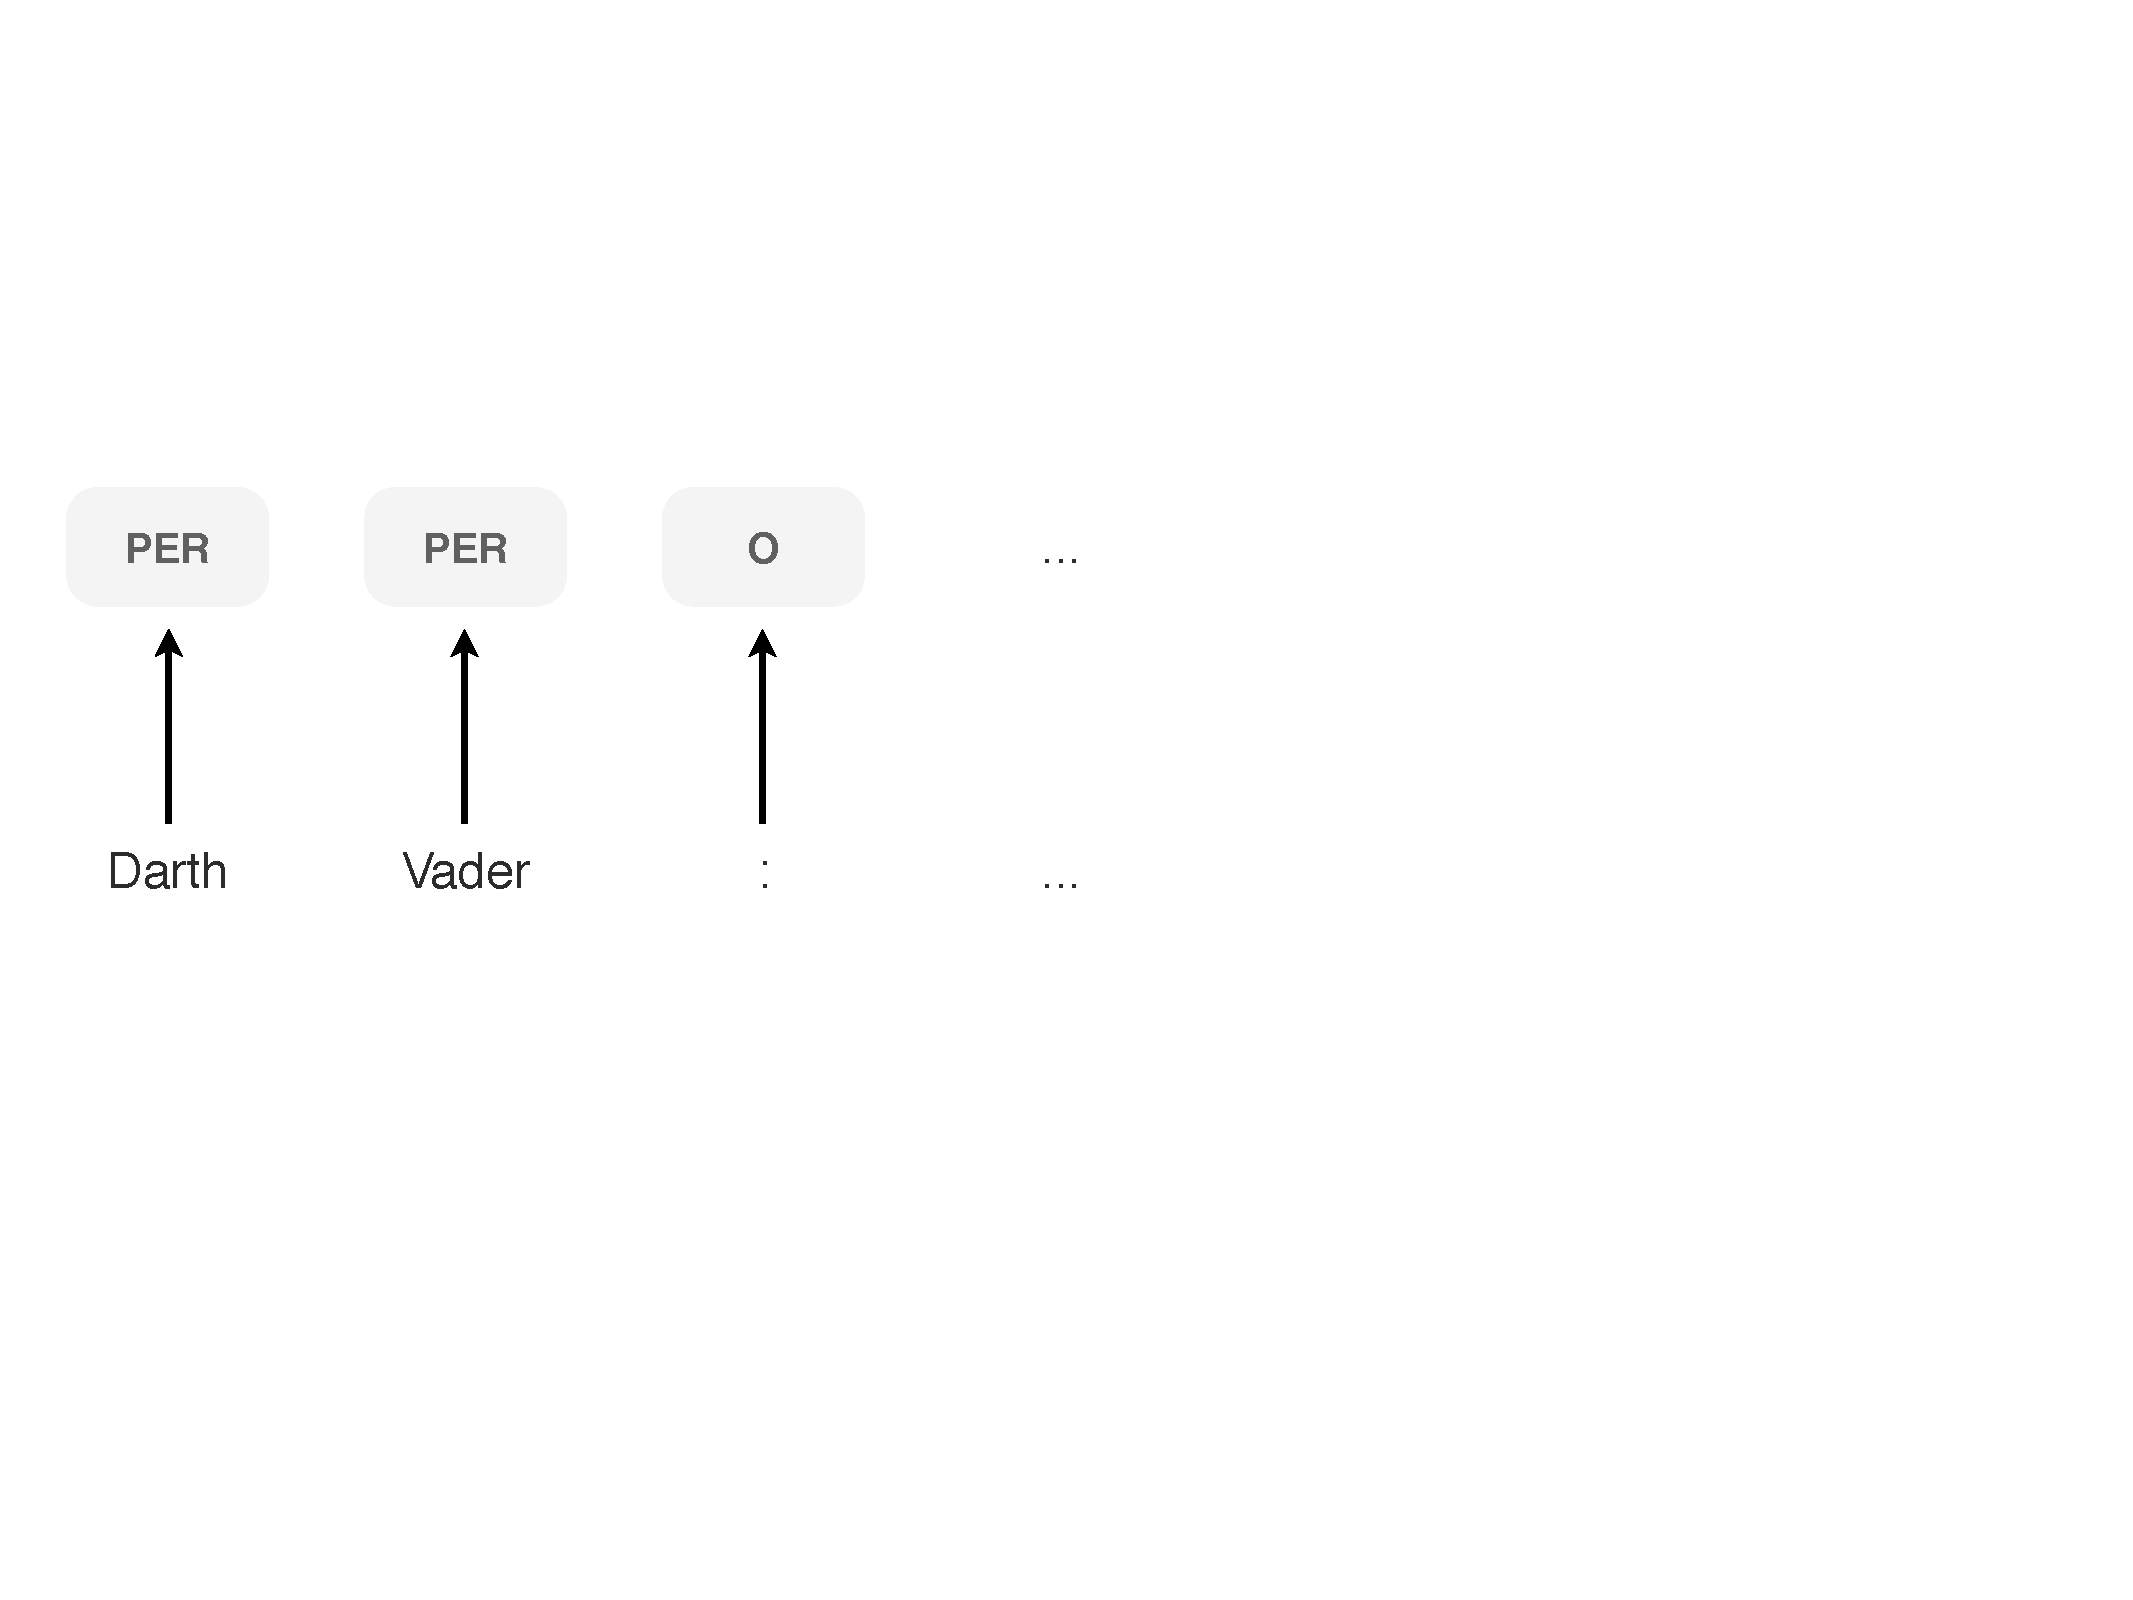
\includegraphics[height=1.6cm, page=1]{figures/local.pdf}
	\end{figure}
	
	Local classifiers
	\small
	\vspace{0.35cm}
	\begin{itemize}
		\item features 
		\item no label interactions
	\end{itemize}
\end{column}

\begin{column}{.3\textwidth}


	\begin{figure}[t]
		\centering
			\includegraphics[height=1.6cm, page=2]{figures/local.pdf}
	\end{figure}

	HMM
	
	\small
	\begin{itemize}
		\item MLE over tokens 
		\item label interaction
	\end{itemize}
\end{column}


\begin{column}{.3\textwidth}
	\begin{figure}[t]
		\centering
			\includegraphics[height=1.56cm, page=3]{figures/local.pdf}
	\end{figure}

	Structured Prediction
	
	\small
	\begin{itemize}
		\item features
		\item label interactions
	\end{itemize}
\end{column}


\end{columns}





\end{frame}


%%%%%%%%%%%%%%%%%%%%%%%%%%%%%%%%%%%%%%%%%%%%%%%%%%%%%%%%%                

\section{Implementation}
\begin{frame}
\frametitle{Our Implementation}

\begin{itemize}
 \item \textbf{Predicted structure:} NE label for each token in the sentence (O if none)
 \item \textbf{Learning:} ~Structured Perceptron with Averaging\\\vspace{0.3cm}\hspace{0.6cm}
	$\displaystyle \mathbf{w} = \frac{\sum_{i = 1...T}{\mathbf{w}^{i}}}{T}$\\ \hspace{0.6cm}where $\mathbf{w}^{i}$ are the weights of epoch $i$
\vspace{0.2cm}


 \item \textbf{Decoding:} Viterbi algorithm (Markov assumption, only 1 prev. label)
 \item implemented in Python using the NumPy package
\end{itemize}
\end{frame}


%%%%%%%%%%%%%%%%%%%%%%%%%%%%%%%%%%%%%%%%%%%%%%%%%%%%%%%%%    

\begin{frame}
\frametitle{Features}

\begin{itemize}
 \item \textbf{Node features}: 
\begin{itemize}
	\item token, suffixes and prefixes (2-4)
	\item number patterns, contains '-', etc. 
	\item Capitalized?, UPPERCASE?
	\item lemma, POS tag
\end{itemize}

 \item \textbf{Label interaction}: 

\begin{itemize}
	\item current and prev. label
	\item current token and last label for prepositions or possessive 's 
\end{itemize}

 \item \textbf{Gazetteer}: 

\begin{itemize}
	\item Mark entities from lists of known names. \emph{Reliability} of each list is learnt by the Perceptron.
	\item Lists are automatically created using a SPARQL query over DBpedia. 
\end{itemize} 
\end{itemize} 
\end{frame}


%%%%%%%%%%%%%%%%%%%%%%%%%%%%%%%%%%%%%%%%%%%%%%%%%%%%%%%%%            


\begin{frame}
\frametitle{Some Challenges}

\begin{itemize}
	\item \textbf{Marking gazetteer entries:}\\
	\begin{itemize}
		\item Directed Acyclic Word Graph (Q: Do I know \texttt{New York .*} ?)
		\item starting at each token, mark longest known entry
	\end{itemize}

 \item \textbf{Headlines and irregular case:}\\\vspace{0.2cm}
\texttt{SOCCER - \underline{BELARUS} BEAT \underline{ESTONIA} IN \underline{WORLD CUP} QUALIFIER .}\vspace{0.1cm}
	\begin{itemize}
		\item useful case information missing
		\item restore most likely case before classification (\emph{truecasing})
	\end{itemize} 
	
\end{itemize} 
\end{frame}



%%%%%%%%%%%%%%%%%%%%%%%%%%%%%%%%%%%%%%%%%%%%%%%%%%%%%%%%%            


\begin{frame}
\frametitle{Evaluation}
\begin{itemize}
	\item \textbf{Training:} error on tokens
	\item \textbf{Evaluation:} Precision and Recall over full Named Entities
	\begin{itemize}
%		\item let $\mathcal{G}$ be the set of gold entities
%		\item let $\mathcal{Y}$ be the set of predicted entities
%		\item $precision = \frac{ | \mathcal{G} \cap \mathcal{Y} | }{ | \mathcal{Y} | }$ 
%		\item $recall = \frac{ | \mathcal{G} \cap \mathcal{Y} | }{ | \mathcal{G} | }$ 



		\item \vspace{0.3cm} $\displaystyle precision =  \frac{  |\,gold\,\cap\,predicted\,| }{ |\,predicted\,| }$ 
		\item \vspace{0.3cm} $\displaystyle recall = \frac{ |\,gold\,\cap\,predicted\,| }{ |\,gold\,| }$ 
		\item \vspace{0.3cm} $\displaystyle F_{1} = \frac{ 2 * precision*recall }{precision + recall} $ 
 

	\end{itemize}

\end{itemize}
\end{frame}



%%%%%%%%%%%%%%%%%%%%%%%%%%%%%%%%%%%%%%%%%%%%%%%%%%%%%%%%%                

\begin{frame}
\frametitle{Results and Conclusion}
\begin{itemize}
\item \textbf{Results (English only)}\\
\begin{tabular}{l c c}
System                & testa & testb\\
\hline
EN (full)             & 0.8109 & 0.7556 \\
EN (no gazetteer)     & 0.7985 & 0.7156\\
\end{tabular} 
\vspace{0.3cm}
\item handling noisy input data important in NER
\item SP is suitable and simple model for NER 
\item reasonable amount of work produces good results 


\end{itemize}
\end{frame}


%%%%%%%%%%%%%%%%%%%%%%%%%%%%%%%%%%%%%%%%%%%%%%%%%%%%%%%%%                

\section*{} % (fold)

\begin{frame}{}
  \begin{center}
\Large    
Thank You!\\

\vspace{0.3cm}
\large
Questions?
  \end{center}
\end{frame}





%% Template

% \section{}
% \begin{frame}
% \frametitle{}
% \end{frame}


%%%%%%%%%%%%%%%%%%%%%%%%%%%%%%%%%%%%%%%%%%%%%%%%%%%%%%%%


\begin{frame}[allowframebreaks]
        \frametitle{References}
        \nocite{*}
        \bibliographystyle{plain}
        \bibliography{ML}
\end{frame}



\end{document}
